% main_kr.tex
\documentclass[11pt,a4paper]{article}

% ---- Language / Font ----
\usepackage[T1]{fontenc}
\usepackage[utf8]{inputenc}
\usepackage{kotex}

% ---- Layout ----
\usepackage[margin=1in]{geometry}
\usepackage{graphicx}
\graphicspath{{../../figures/}}

% ---- Math / Tables ----
\usepackage{amsmath,amssymb}
\usepackage{booktabs}
\usepackage{array}
\usepackage{longtable}

% ---- Lists / Links ----
\usepackage{enumitem}
\usepackage[hidelinks]{hyperref}

% ---- Bibliography ----
\usepackage[numbers]{natbib}

\title{라우팅 공격 환경에서 복원력을 갖춘 신뢰 기반 Backpressure RPL(Trust-Aware BRPL)}
\author{이건형}
\date{}

\begin{document}
\maketitle

\begin{abstract}
Low-Power and Lossy Network(LLN)은 무선 링크 손실과 혼잡(congestion) 상황에서도 안정적인 라우팅이 필요하며, 이를 위해 RPL과 backpressure 기반 변형인 BRPL이 활용된다. 그러나 기존 RPL/BRPL은 내부자 라우팅 공격(insider routing attack)—예를 들어 데이터 평면(data-plane)의 전달(forwarding)을 조작하거나, 제어 평면(control-plane)의 광고(advertisement, 예: rank)를 조작하는 행위—을 명시적으로 고려하지 않는다. 이로 인해 토폴로지와 라우팅 구조에 따라 특정 공격 강도(attack intensity)를 넘으면 성능이 급격히 붕괴(collapse)할 수 있다. 본 문서는 BRPL의 라우팅 결정에 신뢰(trust) 기반 패널티(penalty)를 경량으로 통합한 \emph{Trust-Aware BRPL}을 정리한다. 데이터 평면 신뢰도는 EWMA 기반 평활화를 적용한 Beta 추정기로 모델링하고, 제어 평면 이상 징후는 rank 불일치 및 안정성(stability) 신호로 포착한다. Contiki-NG/Cooja 시뮬레이션에서 공격 강도, 토폴로지 클래스, 네트워크 규모를 스윕(sweep)하는 재현 가능한 실험을 구성하며, BRPL과 Trust-Aware BRPL을 패킷 전달률(PDR), 종단간 지연(end-to-end delay), 제어 오버헤드(control overhead), 부모 변경률(parent churn) 관점에서 비교한다. 결과(추후 삽입)는 신뢰 파라미터가 붕괴 임계값(collapse threshold)을 어떻게 이동시키는지 정량화하고, 복원력(resilience)과 오버헤드 간 트레이드오프(trade-off)를 분석하도록 구성된다.
\end{abstract}

\noindent\textbf{Keywords:} RPL, BRPL, backpressure, trust, LLN, IoT 보안, selective forwarding, sinkhole, Contiki-NG, Cooja

\section{Introduction}
\label{sec:intro}
LLN은 엄격한 전력/메모리 제약(power/memory constraint) 하에서 동작하는 IoT 센싱 및 제어 시스템에 널리 사용되며, 손실이 큰 무선 링크(lossy wireless link)를 통해 통신한다. RPL은 DODAG 형성(DODAG formation), rank, 부모 선택(parent selection)에 기반한 LLN용 표준 IPv6 라우팅 프레임워크를 제공한다 \citep{rfc6550}. BRPL은 backpressure 기반 의사결정을 통해 RPL을 확장하여, 혼잡(congestion) 상황에서 경로 다양성(path diversity)을 활용함으로써 처리율(throughput)과 지연(latency)을 개선한다 \citep{moeller2016brpl}.

그럼에도 LLN 라우팅은 내부자 공격(insider attack)에 취약하다. 대표적인 위협으로 (i) \emph{선택적 전달(selective forwarding)}(grayhole/blackhole) 공격이 있으며, 손상된 전달자(compromised forwarder)가 확률적으로 패킷을 드롭(drop)한다. (ii) \emph{싱크홀(sinkhole)} 공격은 오해를 유발하는 제어 평면 광고(misleading control-plane advertisement, 예: rank 조작)를 통해 트래픽을 유인한 뒤 전달을 방해한다 \citep{karlof2003secure,wood2002dos,le2013rank,mayzaud2016taxonomy}. 경험적으로 이러한 공격은 상전이(phase transition)에 유사한 거동을 보인다. 공격 강도(attack intensity)가 낮을 때는 성능 저하가 제한적이지만, 토폴로지(topology)와 라우팅 구조(routing structure)에 의존하는 임계값(threshold)을 넘어서면 성능이 급격히 붕괴한다.

\subsection{Goal and Approach}
\label{subsec:goal}
본 문서의 목표는 경량 신뢰 신호(lightweight trust signal)를 BRPL의 의사결정 과정(decision process)에 통합하여 이러한 붕괴를 지연시키거나 완화하는 것이다. 무거운 암호 기법(heavy cryptographic mechanism)이나 독립적인 침입 탐지(standalone intrusion detection)를 추가하는 대신, 신뢰를 라우팅 메트릭(routing metric)의 \emph{패널티(penalty)}로 통합한다. 즉, 의심되는 노드는 전달자/부모로서 덜 매력적이 되도록 만들면서도, BRPL의 혼잡 인지(congestion-aware) 장점은 유지하는 방향을 지향한다.

\subsection{Contributions}
\label{subsec:contrib}
\begin{itemize}[leftmargin=*]
  \item \textbf{Trust-Aware BRPL 설계:} backpressure 기반 적응성(adaptivity)을 유지하면서 신뢰도가 낮은 이웃(neighbor)을 down-weight하는 경량 trust-penalized BRPL 메트릭을 정리한다.
  \item \textbf{이중 평면(dual-plane) 신뢰 모델:} 데이터 평면(data-plane) 신뢰는 Beta 추정(Beta estimation) + EWMA 평활화(smoothing)로, 제어 평면(control-plane) 신뢰는 RPL 의미론(semantics)에서 도출한 rank 불일치(inconsistency) 및 안정성(stability) 신호로 모델링한다.
  \item \textbf{재현 가능한 평가 프레임워크:} Contiki-NG/Cooja 구현과 스크립트 기반 스윕(scripted sweep)을 통해 토폴로지 클래스, 규모(scale; S/M/L), 공격 강도를 체계적으로 변화시키며 selective forwarding, sinkhole, 복합(combined) 공격을 평가한다.
  \item \textbf{붕괴 임계값(collapse-threshold) 분석 구성:} 신뢰 파라미터가 붕괴 지점을 어떻게 이동시키는지, 그리고 복원력(resilience)이 오버헤드(overhead) 및 churn과 어떻게 트레이드오프 되는지 정량화하도록 결과를 구성한다.
\end{itemize}

\subsection{문서 구성}
Section~\ref{sec:background}에서는 배경 및 관련 연구를 정리한다.
Section~\ref{sec:model}에서는 시스템/위협 모델을 정의한다.
Section~\ref{sec:design}에서는 Trust-Aware BRPL 설계를 제시한다.
Section~\ref{sec:impl}에서는 구현 사항을 설명한다.
Section~\ref{sec:setup}에서는 실험 설정을 기술한다.
Section~\ref{sec:results} 및 Section~\ref{sec:discussion}에서는 결과 보고 및 논의를 수행한다.
Section~\ref{sec:conclusion}에서 결론을 정리한다.

\section{Background and Related Work}
\label{sec:background}
\subsection{RPL과 BRPL}
RPL은 싱크(sink)를 루트(root)로 하는 DODAG를 구성하고, rank를 사용해 루프 회피(loop avoidance)와 수렴(convergence)을 보장한다 \citep{rfc6550}. BRPL은 backpressure 원리를 RPL에 접목하여 큐 차이(queue differential)와 라우팅 비용(routing cost)을 결합함으로써 혼잡 환경에서 처리율과 지연을 개선하고, 가능한 경우 다중 경로(multi-path)를 활용한다 \citep{moeller2016brpl}.

\subsection{LLN 라우팅 공격}
선택적 전달(selective forwarding) 및 싱크홀/랭크(sinkhole/rank) 공격은 LLN의 전달 성능(delivery)과 안정성(stability)을 크게 저하시킬 수 있는 위협으로 보고되어 왔다 \citep{karlof2003secure,wood2002dos,le2013rank,mayzaud2016taxonomy}. 특히 sinkhole은 오해를 유발하는 제어 평면 정보(misleading control-plane information)로 트래픽을 유인하며, 중요 경로(critical path)에 위치한 이후에는 방해(disruption)를 증폭시키기 쉽다.

\subsection{신뢰 기반 라우팅}
신뢰 기반 라우팅(trust-based routing)은 행동적 신뢰(behavioral reliability)를 라우팅 결정에 반영하는 접근으로, 직접 관찰(direct observation) 및/또는 평판(reputation) 시스템을 활용한다 \citep{ganeriwal2004reputation,ganeriwal2008tosn,momani2010survey}. LLN에서는 무선 관찰의 불완전성 및 overhearing 제약 때문에, full watchdog 방식보다는 경량 추정기(lightweight estimator)와 평활화(smoothing)가 실용적이다.

\section{System and Threat Model}
\label{sec:model}
\subsection{System Model}
Contiki-NG와 Cooja를 사용하여 RPL/BRPL 라우팅이 포함된 6LoWPAN/IPv6 LLN 스택(stack)을 시뮬레이션한다. 트래픽은 센서 노드(sensor node)에서 루트(root)로의 다대일(many-to-one) 주기적(periodic) 패턴을 따른다. 각 노드는 이웃 테이블(neighbor table)을 유지하며, 기반 라우팅 로직(underlying routing logic)에 따라 선호 부모(preferred parent)를 선택한다 \citep{rfc6550,moeller2016brpl}.

\subsection{Threat Model}
단일 내부자 공격자(single insider attacker)를 고려한다(다중 공격자는 향후 과제). 공격자는 정상 노드로 참여하되 다음 중 하나를 수행한다:
\begin{itemize}[leftmargin=*]
  \item \textbf{선택적 전달(selective forwarding):} 전달 중인 트래픽에 대해 확률적 패킷 드롭(probabilistic drop)을 수행하며, 드롭 확률(drop probability)을 공격 강도(attack intensity)로 스윕한다.
  \item \textbf{싱크홀(sinkhole; rank manipulation):} 트래픽 유인을 위해 인위적으로 낮은 rank를 광고(advertise)하는 등 제어 평면을 조작한다. 드롭과 결합되지 않는 경우에는 정상 전달을 수행한다.
  \item \textbf{복합(combined) 공격:} sinkhole로 유인한 이후, 유인된 플로우(captured flow)에 선택적 전달을 결합한다.
\end{itemize}
루트(root)는 악의적이지 않다고 가정한다. 암호 기반 인증(authentication)과 secure bootstrapping은 범위 밖으로 둔다.

\section{Trust-Aware BRPL Design}
\label{sec:design}
본 절에서는 신뢰 신호(trust signal)를 정의하고, 이를 BRPL 결정에 반영하는 방법을 기술한다. 관측 노드를 $i$, 이웃 후보(neighbor candidate; parent/forwarder)를 $j$로 표기한다. 신뢰 값(trust value)은 $[0,1]$로 정규화하며, 값이 클수록 신뢰도가 높다.

\subsection{Data-Plane Trust for Selective Forwarding}
\label{subsec:grayhole}
전달 신뢰도를 이웃이 패킷을 성공적으로 전달할 확률로 모델링한다. $s_j$와 $f_j$는 각각 $j$에 귀속된 전달 성공/실패 이벤트 관측치(예: log-based inference)를 나타낸다. Bernoulli 전달 결과에 대해 Beta 사전분포(prior) $(\alpha_0,\beta_0)$를 적용하면 \citep{ganeriwal2004reputation,ganeriwal2008tosn}, posterior mean은
\begin{equation}
\hat{T}_{\text{gray}}(j)=\frac{\alpha_0+s_j}{\alpha_0+\beta_0+s_j+f_j}
\end{equation}
이다. 단기 잡음(short-term noise)을 줄이기 위해 EWMA 평활화(EWMA smoothing)를 적용한다:
\begin{equation}
T_{\text{gray}}(j;t)=\rho\,T_{\text{gray}}(j;t\!-\!1)+(1-\rho)\,\hat{T}_{\text{gray}}(j),
\end{equation}
여기서 $\rho\in[0,1)$는 평활화 강도를 제어한다.

\subsection{Control-Plane Trust for Sinkhole Behavior}
\label{subsec:sinkhole}
Sinkhole 공격은 주로 제어 평면(control-plane) 광고(advertisement)에 영향을 준다. RPL의 rank 의미론은 가능한 부모 관계(feasible parent relation)에 monotonicity constraint를 부과한다 \citep{rfc6550}. $R_i$를 노드 $i$의 current rank, $R_j$를 이웃 $j$가 광고한 advertised rank로 둔다. 다음을 정의한다:
\begin{equation}
\Delta_{ij}=R_j+\mathrm{MIN\_HOPRANKINC}-R_i.
\end{equation}
$j$가 $i$ 대비 비현실적으로 낮은 rank를 광고하면 $\Delta_{ij}$가 음수가 된다. 허용 오차(tolerance) $\tau\ge 0$를 두고 deviation score를
\begin{equation}
s_{ij}=\max(0,\,-\Delta_{ij}-\tau)
\end{equation}
로 정의한 뒤, exponential trust decay로 매핑한다 \citep{sun2005trust,chen2010trust}:
\begin{equation}
T_{\text{adv}}(j)=\exp(-\lambda_{\text{adv}}\,s_{ij}),
\end{equation}
여기서 $\lambda_{\text{adv}}>0$는 민감도(sensitivity)를 설정한다.

또한 sinkhole은 rank evolution 및 부모 선택(parent selection)의 불안정(instability)을 유발할 수 있다. Window $W$에 대해 rank increase를
\begin{equation}
\Delta R_i=R_i(t)-R_i(t-W)
\end{equation}
로 정의하고, $\kappa\ge 0$를 넘는 비정상 증가(abnormal increase)를 패널티한다:
\begin{equation}
u_i=\max(0,\,\Delta R_i-\kappa), \qquad
T_{\text{stab}}(t)=\exp(-\lambda_{\text{stab}}\,u_i).
\end{equation}
제어 평면 신호(control-plane signal)는 곱셈적으로 결합한다:
\begin{equation}
T_{\text{sink}}(j)=\left(T_{\text{adv}}(j)\right)^{w_1}\left(T_{\text{stab}}(t)\right)^{w_2},
\end{equation}
여기서 $w_1,w_2\ge 0$는 각 신호의 가중치(weight)이다.

\subsection{Total Trust Aggregation}
\label{subsec:totaltrust}
데이터 평면 및 제어 평면 신뢰는 weighted geometric mean으로 집계한다:
\begin{equation}
T_{\text{total}}(j)=\left(T_{\text{gray}}(j)\right)^{\alpha}\left(T_{\text{sink}}(j)\right)^{1-\alpha},
\end{equation}
여기서 $\alpha\in[0,1]$는 selective forwarding과 sinkhole 신호 사이의 강조 비율을 제어한다.

\subsection{Trust-Penalized BRPL Metric}
\label{subsec:metric}
$BP_{ij}$를 노드 $i$에서 이웃 $j$에 대한 baseline BRPL weight/utility로 둔다(BRPL의 backpressure와 cost 결합으로 정의됨) \citep{moeller2016brpl}. Trust penalty factor를
\begin{equation}
\phi(T)=\frac{T^{\gamma}}{1+\lambda\,(1-T)^{\gamma}},
\label{eq:phi}
\end{equation}
로 정의하며, $\lambda\ge 0$는 회피 강도(avoidance aggressiveness), $\gamma\ge 1$은 위험 민감도(risk sensitivity)를 제어한다. Trust-aware metric은
\begin{equation}
BP^{\text{(trust)}}_{ij}=BP_{ij}\cdot \phi\!\left(T_{\text{total}}(j)\right)
\end{equation}
이다. 본 형태는 trust가 균일할 때 ordering을 보존하며, $\lambda$ 또는 $\gamma$가 증가할수록 low-trust neighbor를 더 강하게 down-weight한다. 조정 가능한 패널티 파라미터(tunable penalty parameter)의 사용은 stochastic network optimization의 drift-plus-penalty 및 risk-sensitive control 직관과 부합한다 \citep{neely2010}.

\subsection{Algorithm Outline}
\label{subsec:algo}
각 decision epoch에서 노드 $i$는 다음을 수행한다:
\begin{enumerate}[leftmargin=*]
  \item 신뢰 값(trust value; data-plane 및/또는 control-plane)을 업데이트하고 $[0,1]$로 clamp한다.
  \item 각 이웃 후보 $j$에 대해 $BP^{\text{(trust)}}_{ij}$를 계산한다.
  \item Trust-penalized objective를 최대화하는 선호 부모(preferred parent) 또는 다음 홉(next hop)을 선택하며, churn 감소를 위해 선택적으로 hysteresis를 적용할 수 있다.
\end{enumerate}

\subsection{Overhead}
\label{subsec:overhead}
Trust 유지를 위해 노드당 $O(\deg)$ 값을 저장하며, 여기서 $\deg$는 이웃 차수(neighbor degree)이다. 메트릭 계산은 decision당 $O(\deg)$ 산술 연산을 추가한다. 설계상 추가 제어 패킷(additional control packet)은 요구되지 않으며, 추가 오버헤드는 변경된 routing dynamics(예: parent switching)에서 발생할 수 있다.

\section{Implementation in Contiki-NG}
\label{sec:impl}
Trust-Aware BRPL은 Contiki-NG에서 trust penalty를 BRPL metric computation 및 parent selection path에 통합하는 방식으로 구현한다. Attacker node는
(i) 선택적 전달을 위한 확률적 드롭(probabilistic drop),
(ii) sinkhole을 위한 rank advertisement manipulation,
(iii) 복합(combined) 동작을 지원한다.

라우팅 결정에 사용되는 모든 trust 값은 simulation runtime 동안 각 노드에서 \emph{online}으로 계산되어 즉시 적용된다. 별도로 수행되는 trust engine의 \emph{offline} log-based analysis는 measurement/visualization/reproducibility 목적에 한정되며, offline 결과가 라우팅 결정으로 피드백되는 일은 없다.

재현성을 위해 seed/topology/attack parameter에 대해 batch experiment를 수행하고, Cooja log에서 metric을 추출하는 scripted pipeline을 유지한다. 구현 세부 파일명 및 스크립트는 본문에서는 생략하며, code repository와 함께 artifact로 제공할 수 있다.

\begin{figure}[t]
  \centering
  \includegraphics[width=0.9\linewidth]{architecture.pdf}
  \caption{Software architecture of Trust-Aware BRPL and its integration into the Contiki-NG protocol stack.}
  \label{fig:arch}
\end{figure}

\begin{figure}[t]
  \centering
  \includegraphics[width=0.9\linewidth]{trust_update_flow.pdf}
  \caption{Online trust update and routing decision flow executed at each node during simulation runtime.}
  \label{fig:trust-flow}
\end{figure}

\section{Experimental Setup}
\label{sec:setup}
\subsection{Simulation Environment}
Cooja의 UDGM Distance Loss radio model을 사용한다 \citep{osterlind2006cooja}. 별도로 명시하지 않는 한 simulation은 600\,s 동안 실행되며 warm-up은 120\,s로 둔다. Sensor node는 30\,s마다 root로 periodic traffic을 생성한다. RPL Trickle parameter는 안정성(stability)과 제어 오버헤드(control overhead) 간 trade-off를 고려한 표준 구성을 따른다 \citep{rfc6550}.

\subsection{Topologies and Scales}
서로 다른 경로 다양성(path diversity) regime을 포괄하기 위해 다음 topology \emph{class}를 평가한다:
\begin{itemize}[leftmargin=*]
  \item \textbf{Grid:} 경로 다양성이 높아 attack을 부분적으로 우회할 수 있음.
  \item \textbf{Two-cluster with bottleneck:} bottleneck이 존재하는 constrained cut 구조로, attacker가 bottleneck 근처에 위치할 때 공격 효과가 증폭됨.
  \item \textbf{Corridor/chain:} 경로 다양성이 낮아 낮은 intensity에서도 collapse가 발생할 수 있음.
  \item \textbf{Ring/spokes:} 중간 수준의 다양성으로, root-near 및 mid-path 영향이 두드러짐.
\end{itemize}
네트워크 규모(scale)는 S/M/L(예: root 포함 16/36/64 nodes)로 확장하되, class별 placement rule은 유지한다. Attacker placement는 ad-hoc tuning을 피하기 위해 rule-based selection(예: central relay candidate 또는 bottleneck vicinity)을 따른다.

\begin{figure}[p]
  \centering
  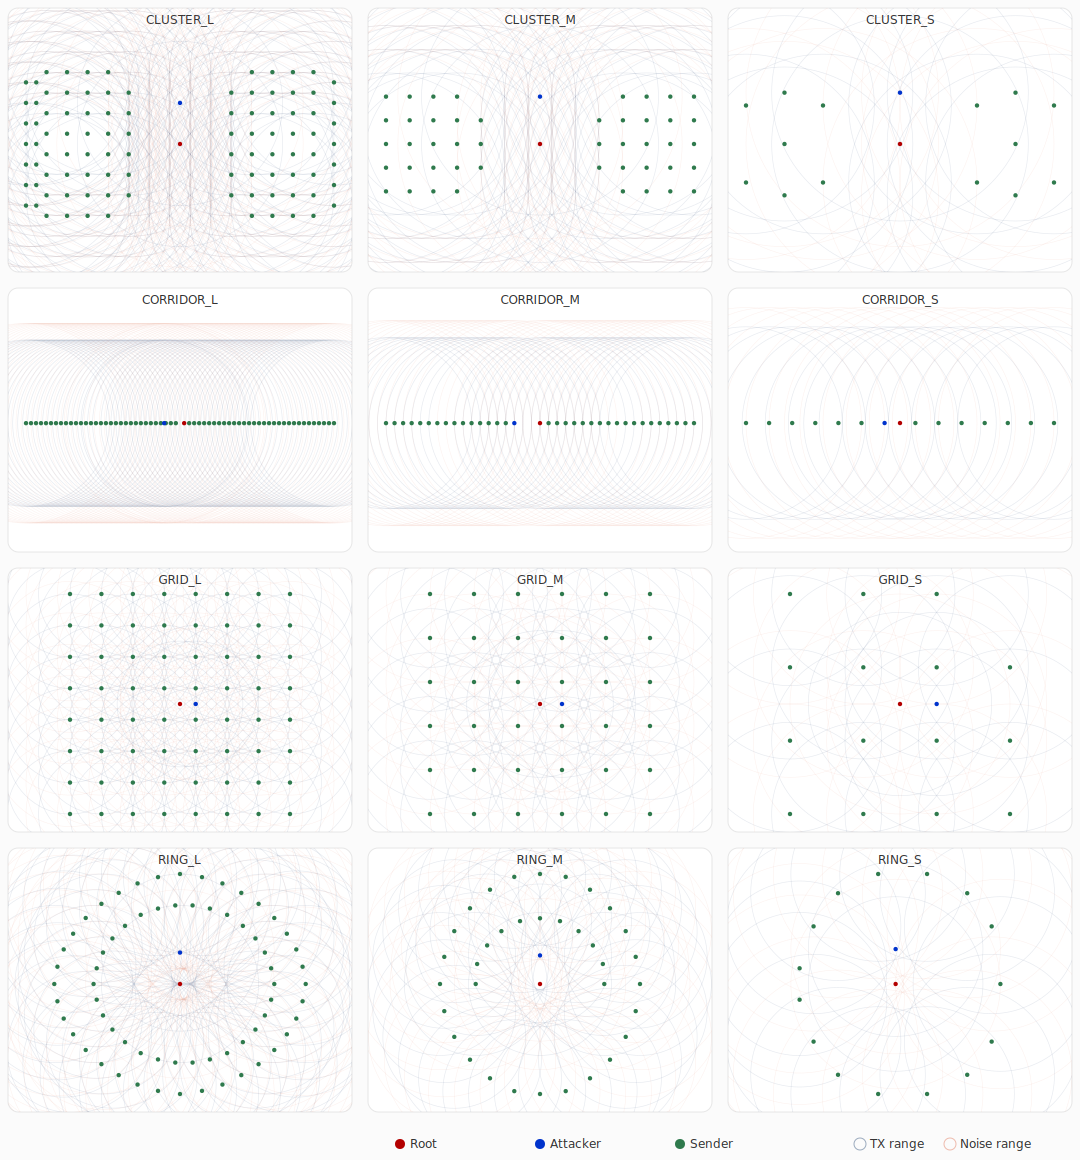
\includegraphics[width=\textwidth,height=\textheight,keepaspectratio]{topology_svgs/all_topologies.pdf}
  \caption{Topology layouts used for evaluation, covering different path diversity regimes and attacker positions.}
  \label{fig:all-topologies}
\end{figure}

\subsection{Attack Configuration}
Selective forwarding은 drop probability(예: 0/30/50/70\%)로 parameterize한다. Sinkhole intensity는 rank manipulation delta(예: 1/2/4)로 parameterize한다. 세 가지 모드를 평가한다: selective forwarding only, sinkhole only, combined.

\begin{figure}[t]
  \centering
  \includegraphics[width=0.9\linewidth]{experiment_workflow.pdf}
  \caption{Experiment workflow from simulation execution to offline metric extraction.}
  \label{fig:workflow}
\end{figure}

\subsection{Trust Model Parameters}
\label{subsec:trust-params}
Table~\ref{tab:trust-params}는 실험 전반에서 사용한 trust 관련 parameter를 요약한다. 별도로 명시하지 않는 한, scenario별 튜닝을 피하기 위해 모든 topology 및 scale에 동일 구성을 적용한다.

\begin{table}[t]
\centering
\caption{Trust model parameters used in experiments.}
\label{tab:trust-params}
\begin{tabular}{lll}
\toprule
Parameter & Description & Value \\
\midrule
$\alpha_0$ & Beta prior (success) & 1 \\
$\beta_0$  & Beta prior (failure) & 1 \\
$\rho$     & EWMA smoothing factor & 0.8 \\
$W$        & Rank stability window & 5 sampling intervals \\
$\tau$     & Rank deviation tolerance & 0 \\
$\kappa$   & Rank increase tolerance & 0 \\
$\lambda_{\text{adv}}$ & Rank anomaly sensitivity & 0.01 \\
$\lambda_{\text{stab}}$ & Rank instability sensitivity & 0.01 \\
$w_1$      & Weight of rank inconsistency trust & 0.5 \\
$w_2$      & Weight of rank stability trust & 0.5 \\
$\alpha$   & Grayhole vs. sinkhole trust weight & \{1.0, 0.5\} \\
$\lambda$  & Trust penalty strength & \{0, 1, 3, 10\} \\
$\gamma$   & Risk sensitivity exponent & \{1, 2, 4\} \\
\bottomrule
\end{tabular}
\end{table}

\subsection{Metrics}
다음 metric을 보고한다:
\begin{itemize}[leftmargin=*]
  \item \textbf{PDR:} $\mathrm{RX}_{\text{root}} / \mathrm{TX}_{\text{senders}}$.
  \item \textbf{종단간 지연(end-to-end delay):} source에서 root까지의 per-packet latency.
  \item \textbf{제어 오버헤드(control overhead):} control-plane transmission(예: DIO/DAO) 및 routing-related overhead.
  \item \textbf{부모 변경률(parent churn):} parent switching rate로, routing stability를 반영.
  \item \textbf{노출(exposure, optional):} delivered packet 중 attacker를 traverse한 비율 및/또는 attacker가 preferred parent인 시간 비율(attack effectiveness 해석용).
\end{itemize}

\subsection{Parameter Sweeps}
다음을 스윕한다:
(i) attack intensity,
(ii) topology class 및 scale,
(iii) trust aggregation weight $\alpha$,
(iv) trust-aware case에 대한 penalty parameter $(\lambda,\gamma)$.
Mean 및 variability를 보고하기 위해 multiple random seed를 사용한다.

\begin{table}[t]
\centering
\caption{Core experimental parameters (default).}
\label{tab:params}
\begin{tabular}{ll}
\toprule
Parameter & Value \\
\midrule
Field size & 200 m $\times$ 200 m \\
Radio model & UDGM Distance Loss \\
TX range / Interference range & 45 m / 90 m \\
Simulation time / Warm-up & 600 s / 120 s \\
Traffic interval & 30 s \\
Root ID & 1 \\
Attacker count & 1 (default) \\
\bottomrule
\end{tabular}
\end{table}

\section{Results}
\label{sec:results}
본 절은 데이터 수집 이후 최종화한다. 분석은 (i) 붕괴 임계값(collapse threshold) 거동과 (ii) trust penalty로 유발되는 trade-off를 강조하도록 구성한다.

\begin{figure}[t]
  \centering
  \fbox{\parbox{0.9\linewidth}{\centering Fig.~3 (placeholder): topology/scale별 attack intensity에 따른 PDR}}
  \caption{PDR vs. attack intensity (placeholder).}
  \label{fig:pdr}
\end{figure}

\begin{figure}[t]
  \centering
  \fbox{\parbox{0.9\linewidth}{\centering Fig.~4 (placeholder): attack intensity에 따른 지연}}
  \caption{End-to-end delay vs. attack intensity (placeholder).}
  \label{fig:delay}
\end{figure}

\begin{figure}[t]
  \centering
  \fbox{\parbox{0.9\linewidth}{\centering Fig.~5 (placeholder): attack intensity에 따른 제어 오버헤드}}
  \caption{Control overhead vs. attack intensity (placeholder).}
  \label{fig:overhead}
\end{figure}

\begin{figure}[t]
  \centering
  \fbox{\parbox{0.9\linewidth}{\centering Fig.~6 (placeholder): attack intensity에 따른 부모 변경률}}
  \caption{Parent churn vs. attack intensity (placeholder).}
  \label{fig:parent-switch}
\end{figure}

\begin{figure}[t]
  \centering
  \fbox{\parbox{0.9\linewidth}{\centering Fig.~7 (placeholder): $(\lambda,\gamma)$ 스윕(sweep) 트레이드오프 표면}}
  \caption{Trade-off under trust penalty sweeps (placeholder).}
  \label{fig:lambda-tradeoff}
\end{figure}

\section{Discussion}
\label{sec:discussion}
본 절에서는 topology-dependent path diversity와 attacker placement가 collapse threshold에 미치는 영향, 그리고 trust penalty가 임계값을 어떻게 이동시키는지 논의한다. 또한 (i) 무선 손실(wireless loss) 및 transient dynamics에서의 false positive 가능성, (ii) $(\lambda,\gamma,\alpha)$에 대한 민감도(sensitivity), (iii) churn 및 overhead에 반영되는 안정성(stability) 영향을 분석한다. 제안 메커니즘은 암호 기반 보호(cryptographic protection) 및 secure bootstrapping을 \emph{대체}하는 것이 아니라 \emph{보완}하기 위한 것으로, full authentication이 불가능하거나 비실용적인 환경에서도 복원력(resilience) 향상을 목표로 한다.

\section{Conclusion and Future Work}
\label{sec:conclusion}
본 문서는 데이터 평면 전달 신뢰(data-plane reliability)와 제어 평면 이상 신호(control-plane anomaly signal)를 함께 활용하여 BRPL 라우팅 결정에 경량 trust penalty를 통합하는 Trust-Aware BRPL을 정리하였다. 평가 설계는 selective forwarding 및 sinkhole 공격 하에서 trust parameter가 성능 붕괴(performance collapse)를 얼마나 지연시키는지 정량화하고, topology 및 scale 전반에서 resilience--overhead trade-off를 특성화하도록 구성된다. 향후 과제로는 colluding multiple attacker, trust penalty parameter의 adaptive tuning, real testbed 검증(validation)을 포함한다.

\bibliographystyle{plainnat}
\bibliography{references}

\end{document}
